% TODO this has a duplicate for some reason
\section{Summarisation Engine}
\label{sec:med42testj}
\subsection{Downloading Models}
All models were downloaded and quantised using the following OpenVINO command:
\begin{verbatim}
    pip install optimum[openvino]
    optimum-cli export openvino --model <huggingface-model-name> 
                --weight-format int4 <output_directory_name>
\end{verbatim}  

\subsection{Testing Models}
To find the model that has the best trade-off between speed and accuracy, the validation set from the previous project was used to created a testing harness to evaluate each model. The \texttt{MTS-Dialog}\cite{mts-dialog} dataset contains 1,700 mock patient-doctor transcripts each with a corresponding medical summary of the conversation, with 170 samples for validation, a strong candidate for evaluating the effectiveness of each model. The dataset was created by 3 Microsoft employees to evaluate Facebook's BART-large \cite{bart} and Google's Pegasus \cite{pegasus} models fine-tuned with guided summarisation and data augmentation. 

\subsubsection{Methodology}
\label{di:test_med42}
I used the Mistral-7b, BioMistral-7b and Med42-v2-8B models for testing based on guidance from my external supervisor. Each model followed the same strategy 
\begin{enumerate}
    \item The model was quantised to int4 and was configured with \texttt{temperature=0.3} \cite{med42temp}
    \item For each validation sample, the ground truth summary, generated summary, and time taken was recorded, then saved to a CSV.
    \item BERT score was used to determine the F1, Precision, Recall metrics explained in \cite{zhang2019bertscore} to quantitatively compare the semantic accuracy of the generated summarisation against the ground truth
    \item The average time was calculated and included in the results
\end{enumerate}

This enabled a comparison between 2 key results: the inference time and accuracy. The results are as follows

\begin{figure}[H]
    \centering
    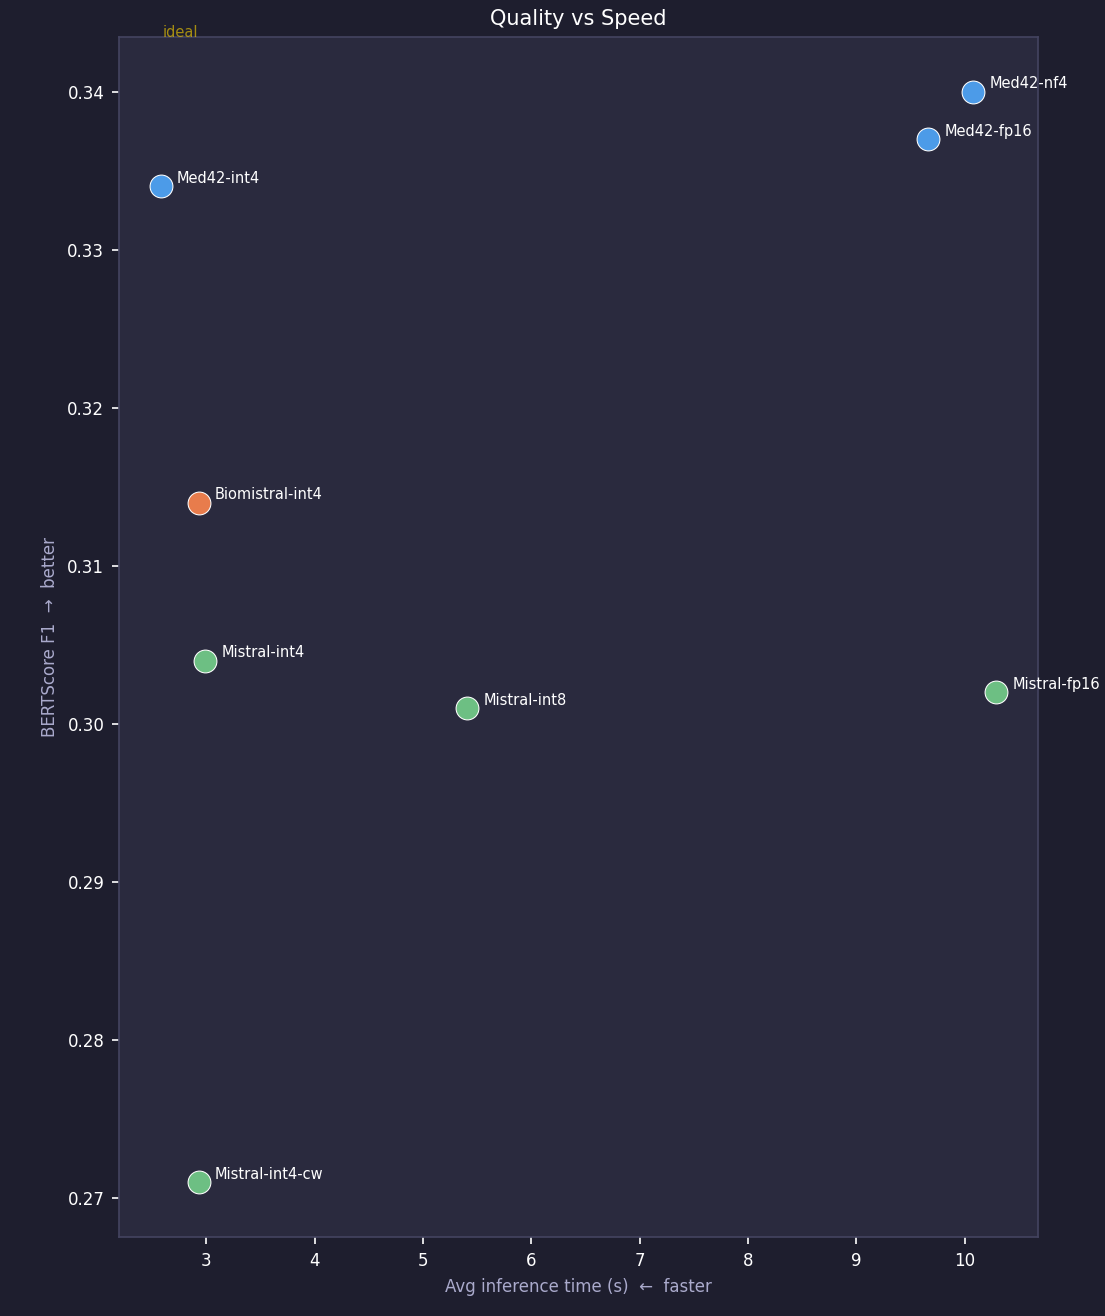
\includegraphics[width=0.75\linewidth]{model_comparison_results.png}
    \caption{A comparison between 3 models with varying quantisation levels, finding the optimal speed-accuracy tradeoff}
    \label{fig:model_comparison_results.png}
\end{figure}

We can conclude that the optimal model for this application is the Med42-v2-8B quantised to int4. As a benefit, the size of the Med42 model was reduced from 19.3GB to 4.3GB on disk.

Further testing on different devices shows the benefit of loading and running the model on the more powerful GPU compared to the NPU, resulting in the GPU being chosen for this component
\begin{figure}[htbp]
    \centering
    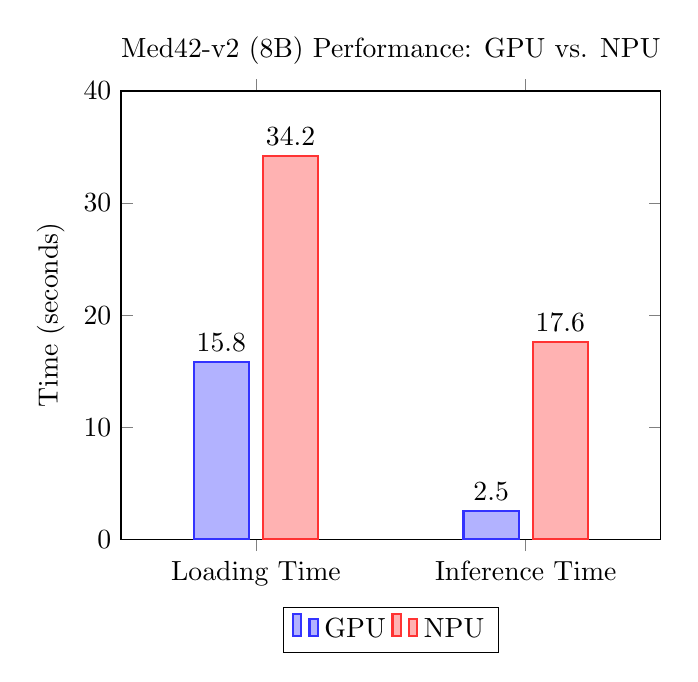
\begin{tikzpicture}
        \begin{axis}[
            ybar=5pt, % Space between the bars in a group
            bar width=20pt, % Width of the bars
            enlarge x limits=0.5, % Padding on the left and right of the chart
            legend style={at={(0.5,-0.15)}, anchor=north, legend columns=-1},
            ylabel={Time (seconds)},
            symbolic x coords={Loading Time, Inference Time}, % Swapped to be the main categories
            xtick=data,
            nodes near coords, % Displays the exact values above the bars
            nodes near coords align={vertical},
            ymin=0, ymax=40, % Normalized the height to fit the new max value (34.2)
            title={Med42-v2 (8B) Performance: GPU vs. NPU}
        ]
        
        % GPU Data (Loading, then Inference)
        \addplot[fill=blue!30, draw=blue!80, thick] coordinates {(Loading Time, 15.8) (Inference Time, 2.5)};
        
        % NPU Data (Loading, then Inference)
        \addplot[fill=red!30, draw=red!80, thick] coordinates {(Loading Time, 34.2) (Inference Time, 17.6)};
        
        \legend{GPU, NPU} % Legend now represents the hardware
        \end{axis}
    \end{tikzpicture}
    \caption{Comparison of loading and inference times for the Med42-v2 8B parameter model running on a GPU versus an NPU.}
    \label{fig:gpu_npu_performance}
\end{figure}


\subsection{Design}
\subsubsection{Concurrency}
The Med42 model requiring 20 seconds to load presents a concurrency constraint. Simply loading this model on the UI thread would cause unacceptable UI latency, therefore the following concurrency design was followed:

\begin{itemize}
    \item At program launch, a background initialisation thread is spawned to load the transcription model
    \item Once the transcription model is ready, this thread launches the Med42 summarisation model asynchronously via \texttt{std::async}, storing the result handle in a shared \texttt{std::future} member (\texttt{m\_summariserLoadFuture})
    \item An atomic boolean flag \texttt{m\_isSummariserReady} is shared between threads and set to \texttt{true} inside the async task once loading completes
    \item When the user starts recording, a separate processing thread is spawned and detached, which calls \texttt{ProcessLoop()} blocking until recording stops
    \item Once recording completes, the processing thread inspects \texttt{m\_isSummariserReady}
    \item If the model has already loaded (the common case where transcription takes longer than 20 seconds), the processing thread proceeds immediately to summary generation
    \item If the model has not yet loaded, the processing thread blocks by calling \texttt{m\_summariserLoadFuture.wait()} until the async loading task completes
    \item Once the summary is generated, the result is marshalled back to the UI thread via \texttt{DispatcherQueue().TryEnqueue()} to display
\end{itemize}

This design handles the race condition where the model has not finished loading but a transcription result arrives. Using \texttt{std::async} and \texttt{std::future} over a raw \texttt{std::thread} is preferred here because \texttt{std::future} provides a first-class blocking synchronisation primitive. The processing thread can call \texttt{wait()} directly on the future without requiring a manually managed \texttt{std::promise} or condition variable, resulting in cleaner synchronisation code.

\subsubsection{Prompting}
The effectiveness of an LLM response is highly linked to the prompt length and detail. Although pre-trained on medical textbooks and guidance, the prompt must still guide the LLM to remove any unecessary conversation and summarise only the medical facts stated to provide a history of present illness summarisation. A consultation with Dr. Tazeen Ahmed determined what was required of the summarisation resulting in the following requirements:
\begin{itemize}
    \item Facts and events must be attributed to "the doctor" or "the patient" with dates in the format DD/MM/YYYY
    \item History must be presented chronologically including onset, duration and character of pain
    \item Specific causes of injury, character of pain, aggravating factors, prior treatments and recent exacerbations must be reported
\end{itemize}

\subsection{Implementation}
The implementation is found in \texttt{SummarisationEngine.cpp}, which wraps the OpenVINO LLM pipeline with \texttt{loadModel()} and \texttt{generateFromTranscription()}

\subsubsection{Model Loading at Launch}
To launch the future from the transcription processing thread, the following implementation was chosen
\begin{verbatim}
m_summariserLoadFuture = std::async(std::launch::async, [this]() {
    try {
        m_summariser->loadModel();
        m_isSummariserReady = true;
    }
    catch (...) {
        MainWindow::SetAppState(AppState::IncompatibleDevice);
    }
});
\end{verbatim}

\texttt{std::launch::async} ensures a real OS thread is spawned. The returned \texttt{std::future<void>} is stored in the \texttt{MainWindow} member \texttt{m\_summariserLoadFuture} blocking summarisation until the task completes preventing the transcription pipeline triggering a summarisation inference before the model loads

Once loaded, the \texttt{std::atomic<bool> m\_isSummariserReady} flag is set to \texttt{true}. Should \texttt{loadModel()} throw when loading, the exception is caught and the application is moved to an \texttt{IncompatibleDevice} error state. Although the \texttt{catch} handles all error types, the only possible error when loading is a device is too little RAM or a non-Intel GPU.

\subsubsection{Waiting for the Model at Summary Time}
Once a final transcript is available, the processing thread must ensure the model is ready before calling \texttt{generateTranscription()}. It does this in two steps:

\begin{verbatim}
if (!m_isSummariserReady) {
    if (m_summariserLoadFuture.valid())
        m_summariserLoadFuture.wait();
}
\end{verbatim}

First, the atomic flag \texttt{m\_isSummariserReady} is checked. Because \texttt{std::atomic} reads are lock-free, this check is extremely cheap and covers the common case where a typical consultation lasts several minutes, well beyond the 20-second load time, so the model will almost always already be ready. If it is, execution proceeds immediately with no synchronisation overhead.

If the flag is still \texttt{false}, the thread falls through to \texttt{m\_summariserLoadFuture.wait()}. The \texttt{.valid()} guard is necessary because a default-constructed \texttt{std::future} has no associated state; calling \texttt{.wait()} on it would be undefined behaviour. \texttt{.wait()} then puts the processing thread to sleep, with no busy-waiting, until the OS wakes it once \texttt{loadModel()} returns. Critically, the UI thread is never involved in any of this waiting.

\subsubsection{Generating and Returning the Summary}
With the model guaranteed to be loaded, \texttt{generateFromTranscription()} is called synchronously on the processing thread. Once the summary string is returned, \texttt{DispatcherQueue().TryEnqueue()} marshals the result back to the UI thread for a UI update.

\subsubsection{Prompting}
The full prompt can be found in Appendix \ref{app:prompt}

